% !TEX TS-program = xelatex
% !BIB program = biber
% !TEX encoding = UTF-8 Unicode

% 使用手冊請見 TW_Thesis_Template wiki:
% https://github.com/sppmg/TW_Thesis_Template/wiki

% User guide in wiki of TW_Thesis_Template :
% https://github.com/sppmg/TW_Thesis_Template/wiki

\documentclass[]{NTHU_thesis} % \documentclass[option1, option2, ...]
% Helpful options: 
% draft = Don't load figure ,reduce compile time.
% showframe = show document margins.
% colorgrid = show colored coordinate. (by eso-pic pkg.)
\usepackage[subpreambles]{standalone} % standalone class setting in config.tex
% Option ``subpreambles'' enable sub-tex's preambles when compile main tex. (pkg default disable)
% sppmg think it's still some problem (e.g. \addbibresource will faild ), recommend move all subpreambles to ``macros_preamble.tex``

\begin{document}
    \frontmatter
        \startWatermark         % 由此開始每頁浮水印
        \documentclass[class=NTHU_thesis, crop=false, float=true]{standalone}
\begin{document}
% I use LaTeX3 to automatically generate name table. 
% Below \ExplSyntaxOn to \ExplSyntaxOff perpare prof. table contents,
% it will save contents to `\profsTableContent''. 
% You can ignore this block even you want make table by yourself.
\ExplSyntaxOn
% Copy prof. list from config.tex
\clist_gclear_new:N \g_sppmg_profsZh_cl
\clist_gset:NV \g_sppmg_profsZh_cl \profsZh
\clist_gclear_new:N \g_sppmg_profsEn_cl
\clist_gset:NV \g_sppmg_profsEn_cl \profsEn

% get total number of prof. . Omitted language will not display.
\int_gzero_new:N \g_sppmg_profTotal_int
\int_gset:Nn \g_sppmg_profTotal_int {
    \int_max:nn {\clist_count:N \g_sppmg_profsZh_cl} 
        {\clist_count:N \g_sppmg_profsEn_cl}
}

% NOTE: ``tabularx'' will  processes its contents more than once 
% for calculate width, so ``gpop'' can't put in tabularx env.
% \tl_if_exist:NTF {\tl_clear:N \g_sppmg_tableContent_tl} {\tl_new:N \g_sppmg_tableContent_tl}
% \tl_if_exist:NTF \g_sppmg_tableContent_tl {} {\tl_new:N \g_sppmg_tableContent_tl}
\tl_gclear_new:N \g_sppmg_tableContent_tl


% Use a inline function for pop 2 list (zh+en), and save table content 
% Input(#1) switch 3 case, 1 = Advisor, 2 = committee member , 3+ is more.
% Use ``for'' loop to get all prof.
\int_step_inline:nnnn {1}{1}{\g_sppmg_profTotal_int}{
    \clist_gpop:NNTF \g_sppmg_profsZh_cl \l_tmpa_tl {}{ \tl_clear:N \l_tmpa_tl}
    \clist_gpop:NNTF \g_sppmg_profsEn_cl \l_tmpb_tl {}{ \tl_clear:N \l_tmpb_tl}
    \tl_gput_right:Nx \g_sppmg_tableContent_tl {
        \int_case:nnTF {#1}{
            {1} {指導教授: & \l_tmpa_tl & 博士 & (Prof.~ \l_tmpb_tl ) \exp_not:n {\\} }
            {2} {共同指導: & \l_tmpa_tl & 博士 & (Prof.~ \l_tmpb_tl ) \exp_not:n {\\} }
        }{}{
            & \l_tmpa_tl & 博士 & (Prof.~ \l_tmpb_tl ) \exp_not:n {\\} 
        }
    }
}

% Copy contents to LaTeX2e macro.
\cs_set_eq:NN \profsTableContent \g_sppmg_tableContent_tl

\ExplSyntaxOff
\def\fsUniversity{\fs{24}[1.5]}
\def\fsTitle{\fs{20}[1.5]}
\def\fsNames{\fs{18}[1.5]}

\def\mcShift{\hspace{-6.0pt}} % It's for align non-multicolumn cell .
% --------define title page layout for thesis
\titlepageFontFamily % set in config.tex
\newgeometry{top=2.5cm, bottom=2.5cm, inner=2cm, outer=2cm} % only for titlepage
\begin{spacing}{1.0}
\begin{titlepage}
    \null\vfill
    \begin{center}
        {\fsUniversity 國\quad 立\quad 清\quad 華\quad 大\quad 學} \par
        \vspace*{5mm}
        
        {\fsTitle {\degree}論文\par}
        \vspace*{20mm}
        
        {\fsTitle {\title} \par}
        \vspace*{5mm}
        
        {\fsTitle {\subtitle} \par}
        \vspace*{10mm}
        
        {\ifx \logo\empty\vspace*{30mm}
        \else \includegraphics[height=30mm]{\logo} \par
        \fi}
        \vfill
        
        {\fsNames \renewcommand{\arraystretch}{1}
            % If you want make table by yourself, replace ``\profsTableContent''
            \begin{tabular}{l@{\hspace*{0.4em}}l@{\quad}l@{\quad}l}
            系\qquad 所: & \multicolumn{3}{l}{\mcShift \dept}      \\
            學\qquad 號: & \multicolumn{3}{l}{\mcShift \studentID} \\
            研\enspace 究\enspace 生: & \authorZh & & (\authorEn)    \\
            
            \profsTableContent
            
            \end{tabular}
        \par}
        \vspace*{5ex}
        
        {\fsTitle {\degreedate} \par}
        \vspace*{2ex}
        
        \ifthenelse{\boolean{printcopyright}}
        {{{版權所有\copyright\ \author\ \quad \copyyear} \par}}
        {}
    \end{center}
    \null\vfill
\end{titlepage}
\end{spacing}
\restoregeometry
\normalfont % use main font
%--------end of title page for thesis
\cleardoublepage
\end{document}
       % 封面/書名頁
        \listoftodos   % todo list, hide when set \textbackslash{}setboolean\{publish\}\{\textbf{true}\} in config.tex. It will not add to TOC , you can add \todototoc before \listoftodos to do that.
            \todoInfo{explain transverse}
            \todoInfo{abbreviation}
            \todoInfo{eta, phi, R definition}
            \todoInfo{add the study introduction in Chapter 1}
            \todoInfo{add references}
            \todoUnsure{Unsure}
            \todoChange{Change}
            \todoInfo{Information}
            \todo[inline]{Inline}
            \missingfigure{Big Warning}

        %%%%%%%%%%%% letters %%%%%%%%%%%%
        % Set file name in config.tex
        % 依校方規定,此處須插入:
        % [v] 清大(電子授權書) 必備,不論是否授權都要裝訂
        % [v] 清大(紙本授權書) 必備,不論是否授權都要裝訂
        % [x] 國家圖書館(電子授權書) 有授權才要裝訂
        % [v] 國家圖書館(紙本論文延後公開/下架申請書)→紙本論文有申請延後公開才要裝訂
        % [v] 指導教授推薦書
        % [v] 考試委員審定書
        % !!! [x] 部份請自行插入

        % 碩博士論文電子檔授權書 Authorization Letter (for electronic)
        \IfFileExists{\letterAuthEl}{
            \cleardoublepage        % 由下個右頁開始
            \includepdf{\letterAuthEl}}{}
        % 碩博士論文紙本授權書 Authorization Letter (for paper)
        \IfFileExists{\letterAuthPa}{
            \cleardoublepage        % 由下個右頁開始
            \includepdf{\letterAuthPa}}{}
        % 國家圖書館(電子授權書) 有授權才要裝訂

        % 碩博士紙本論文延後公開/下架申請書。(如需延後公開者,才需要裝訂於論文內頁)
        \IfFileExists{\letterPubReq}{
            \cleardoublepage
            \includepdf{\letterPubReq}}{}
        % 指導教授推薦書
        \IfFileExists{\letterRecom}{
            \cleardoublepage
            \includepdf{\letterRecom}}{}
        % 口試委員審定書
        \IfFileExists{\letterVerif}{
            \cleardoublepage
            \includepdf{\letterVerif}}{}
        \cleardoublepage
        
        %%%%%%%%%%%% Other frontmatter, eg,abstract %%%%%%%%%%%%
        % 中英文論文摘要:內容應說明研究目的,資料來源,研究方法及研究結果等
        \documentclass[class=NTHU_thesis, crop=false]{standalone}
\begin{document}
\setlength{\parindent}{2em} %縮排2字寬

\chapter{摘要}
在利用衰變成一對底夸克對的希格斯粒子,來尋找與其相伴產生$Z^\prime$-2HDM模型的暗物質分析中,最後的擬合使用了$Z$玻色子衰變成兩個輕子的分布,來估計$Z$玻色子衰變成兩個微中子的背景。在過去的分析中是以舊有的分布比例當作參數,而在本論文中使用了最新的蒙地卡羅樣本衰變比例以增進分析結果。

\vspace{2em}
\noindent \textbf{關鍵字:} \keywordsZh{} % Set keywords in config.tex
\end{document} % zh 中文摘要
        \documentclass[class=NTHU_thesis, crop=false]{standalone}
\begin{document}

\chapter{Abstract}
In the search for the dark matter of the $Z^\prime$-2HDM model produced in association with a Higgs boson decaying to $b\bar{b}$, the kinematics of $Z \to ll$ are used to estimate $Z \to \nu\nu$, the main background of the process in the post-fit stage. Instead of using the ratio of the $Z \to \nu\nu$ decay channel to $Z \to ll$ decay channel based on the previous analysis, this thesis presents the improvement of the analysis by using the ratio of the updated Monte-Carlo (MC) samples of the $Z$ boson.

\vspace{2em}
\noindent \textbf{Keywords:} \keywordsEn{} % Set keywords in config.tex
\end{document} % en 英文摘要
        \documentclass[class=NTHU_thesis, crop=false]{standalone}
\begin{document}

\chapter{Acknowledgements}
感謝指導教授徐百嫻教授的辛勤指導。這段時間如沐春風,教授仰之彌高,鑽之彌堅。
\newline

感謝Patrick Rieck博士和Samuel Meehan博士給我這份難得可貴的機會,讓我參與這個分析。
\newline

感謝Philipp Gadow博士與呂昀儒博士,當我在程式編碼上遇到困難時,給了我大量的協助。
\newline

感謝韓正忻以及組內的其他人,是這份論文的分析一路下來的工作搭檔。
\newline

最後感謝媽媽全力支持,即使我的人生規劃和她所預期的有些出入。

\end{document}


 % 誌謝(可略)

        % 原始 book class 不將 TOC,LOF,LOT 加入目錄列表,須手動加
        % 此樣板可由 config.tex 切換是否自動加入目錄
        \tableofcontents        % 目錄
        \listoffigures          % 圖目錄
        \listoftables           % 表目錄
        \documentclass[class=NTHU_thesis, crop=false]{standalone}
\begin{document}

\chapter{Glossary}
Use table for symbol list. You can also use package ``nomencl'' (simple) or ``glossaries'' (powerful). see packages document or my tutorial (but it's Chinese).

\begin{table}[h]
    \normalsize
    \centering
    \begin{tabular}{c@{\quad:\quad}l}
%         Symbol  & Description \\ 
        VIM     & The best guy's editor \\ 
        Emacs   & The God's editor \\ 
        CTAN    & Comprehensive TeX Archive Network, ctan.org \\
        
    \end{tabular} 
    \caption*{Glossary} % Hide caption by comment/remove it, label will inactive also. 不想顯示請註解/刪除\caption行(\label自動失效)
    \label{table:glossary_def}
\end{table}

\end{document}
    % 符號說明
    \mainmatter
        \documentclass[class=NTHU_thesis, crop=false]{standalone}
\begin{document}


\chapter{Introduction}
In the universe, the galaxies are observed to violate Newton's second law with the rotation of the observable matters which is faster than expected. Thus it is thought that there are invisible matters called Dark Matter (DM) generating additional gravity to accelerate the rotation. The most popular hypothesis is proposed that DM is a stable and electrically natural particle $\chi$ which only has weak and gravitational interaction with the Standard Model (SM) particles. Thanks to the characteristics, we can try to search such particle at the Large Hadron Collider (LHC).

One possible model of DM is a Type-II two-Higgs-doublet model (2HDM) with an additional U(1)$_{Z^\prime}$ gauge symmetry, known as the $Z^\prime$-2HDM model. A light scalar $h$, which is identified as the SM Higgs boson, and a pseudo-scalar $A$ are introduced among this model, together with a striking process shown in \cref{fig:DM-Model}. The process has the attribute targeted by the collider searches that the final state is DM following with a detectable particle, the SM Higgs boson $h$ in this case. Due to the single visible Higgs boson in the final state, the search for DM of $Z^\prime$-2HDM model is called the monoH analysis. This analysis exploits the largest decay branching ratio of a Higgs boson into a pair of $b$-quarks.

\fig[0.45][fig:DM-Model][!hbt]{DM-Model.png}[The aimed process of the production of DM $\chi$ in the $Z^\prime$-2HDM model. A SM Higgs boson decaying to a pair of $b$-quarks is produced through a $Z^\prime$ mediator coupled to a pseudo-scalar Higgs boson $A$, which eventually decays to undetectable $\chi\bar{\chi}$.]

\end{document}    % 緒論
        \documentclass[class=NTHU_thesis, crop=false]{standalone}
\begin{document}

\chapter{ATLAS Detector}
\label{chap:ATLAS_Detector}
The ATLAS (A Toroidal LHC ApparatuS) \cite{1748-0221-3-08-S08003} is a multifunctional detector with a nominally forward-backward symmetric cylindrical geometry with respect to the interaction point. It comprises four detector components which are the inner detector tracking system, the electromagnetic (EM) calorimeter, the hadronic calorimeter and the muon spectrometer. The overview of the ATLAS is shown in \Cref{fig:ATLAS}.

\fig[0.7][fig:ATLAS][!hbt]{ATLAS.jpg}[The overview of the ATLAS.]

The inner detector is composed of three sub-detectors, the silicon pixel layers, the silicon microstrip (SCT) layers and the transition radiation tracker (TRT), shown in \Cref{fig:ID}. The silicon pixels and the SCT are placed in the range of $\left|\eta\right| < 2.5$, providing the information of pattern recognition, outstanding momentum resolution and both primary and secondary vertex measurements. The TRT comprises many layers of gaseous straw-tube tracking detectors in the range of $\left|\eta\right| < 2.0$, taking charge of continuous charged-particle tracks to improve the pattern recognition and enhance the momentum resolution and also giving the electron identification.

\fig[0.7][fig:ID][!hbt]{ID.jpg}[The schematic diagram of the ATLAS inner detector, which comprises three sub-components, pixels, SCT and TRT. Besides the three pixel layers shown in the figure, there is also a newly added layer, the Insertable B-Layer (IBL) \cite{Capeans:1291633}, as the innermost silicon pixel, improving the identification of displaced vertices and the $b$-tagging performance.]

The calorimeters measure electron, photon, jet and $\tau$ lepton energies, covering the range of $\left|\eta\right| < 4.9$, shown in \Cref{fig:Calorimeter}. The EM calorimeters are liquid argon (LAr) detectors which are accommodated in three cryostats, two end-caps and one barrel, covering the range of $\left|\eta\right| < 3.2$. The LAr is used because of its inherent behavior, stability of response over time and intrinsic radiation-hardness.

Outside the EM calorimeter envelope, the hadronic calorimeter can be divided into the LAr hadronic end-cap calorimeters, the LAr forward calorimeters and the tile calorimeters for the range of $\left|\eta\right| < 4.9$. The LAr hadronic end-cap calorimeters cover the range of $1.5 < \left|\eta\right| < 3.2$, sharing the cryostats with the EM end-cap calorimeters and the forward calorimeters. The LAr forward calorimeters are placed in the range of $3.1 < \left|\eta\right| < 4.9$. As mentioned previously, the LAr is chosen for its inherent excellent property. The tile calorimeters consist of one central barrel calorimeter and two extended barrel calorimeters, made of steel as the absorber and scintillating tiles as the active material, laying over the range of $\left|\eta\right| < 1.7$.

\fig[0.8][fig:Calorimeter][!hbt]{Calorimeter.jpg}[The schematic diagram of the calorimeters, composed of the EM calorimeter and the hadronic calorimeter.]

The outmost component is the muon spectrometer. Over the range of $\left|\eta\right| < 2.7$, the high-precision tracking chambers measure muon tracks in the large superconducting air-core toroid magnets. There are also the trigger chambers covering the range of $\left|\eta\right| < 2.4$ for providing bunch-crossing identification, providing well-defined $p_T$ thresholds, and measuring the muon coordinate in the direction orthogonal to that determined by the precision-tracking system.

The superconducting magnetic system is significantly featured in the ATLAS. As shown in \Cref{fig:ATLAS}, the magnet system consists of one solenoid magnet, one barrel toroid magnet and two end-cap toroid magnets. The solenoid magnet gives $2\, \mathrm{T}$ magnetic field for the inner detector, bending the tracks of charged particles for the momentum measurement and minimizing the radiative density in front of the barrel EM calorimeter. The barrel toroid magnet and the end-cap toroid magnets produce a $0.5\, \mathrm{T}$ and $1\, \mathrm{T}$ toroidal magnetic field in the central and end-cap regions respectively, supplying the bending power for the muon detectors.

Because of the cylindrical structure, all the directional physical quantities used in the analysis are transverse. Apart from the azimuthal angle $\phi$ and the angle between the momentum and the the beam axis $\theta$, some geometrical variables are also defined. The pseudorapidity $\eta$ describes the angle of a particle relative to the beam axis, defined as $\eta = -\ln[\tan(\theta/2)]$. In addition, the rapidity $R$ is used for a measure of angular separation between particles, defined as $R = \sqrt{(\Delta\eta)^2 + (\Delta\phi)^2}$.

Apart from the detector structure, there are also the trigger system carrying out the event selection. There are up to one billion proton-proton collisions per second in the ATLAS and the trigger system only selects 100 events worth retaining per second. There are three levels for the selection process. The Level-1 trigger searches for high $p_T$ muons, electrons, photons, jets, $\tau$ leptons and large missing and total transverse energy. The Level-2 trigger tags these events with some specific regions of interest, leaving below 3500 events per second. In the end, approximately 200 events after the Level-3 trigger.
\end{document}          % 分析方法
        \documentclass[class=NTHU_thesis, crop=false]{standalone}
\begin{document}

\chapter{Review on the MonoH Analysis}
\section{Dark Matter and the $Z^\prime$-2HDM Model}
In the universe, the galaxies are observed to violate Newton's second law with the rotation of the observable matters which is faster than expected. Thus it is thought that there are invisible matters called Dark Matter (DM) generating additional gravity to accelerate the rotation. The most popular hypothesis is proposed that DM is a stable and electrically natural particle $\chi$ which only has weak and gravitational interaction with the Standard Model (SM) particles. Thanks to the characteristics, we can try to search such particle at the Large Hadron Collider (LHC).

One possible model of DM is a Type-II two-Higgs-doublet model (2HDM) with an additional U(1)$_{Z^\prime}$ gauge symmetry, known as the $Z^\prime$-2HDM model. A light scalar $h$, which is identified as the SM Higgs boson, and a pseudo-scalar $A$ are introduced among this model, together with a striking process shown in Figure 3.1. The process has the attribute targeted by the collider searches that the final state is DM following with a detectable particle, the SM Higgs boson $h$ in this case. Due to the single visible Higgs boson in the final state, the search for DM of $Z^\prime$-2HDM model is called the monoH analysis. This analysis exploits the largest decay branching ratio of a Higgs boson into a pair of b-quarks. The following sections will briefly present the result of the analysis.

\fig[0.45][!hbt]{DM-Model.png}[The aimed process of the production of DM $\chi$ in the $Z^\prime$-2HDM model. A SM Higgs boson decaying to a pair of $b$ quarks is produced through a $Z^\prime$ mediator coupled to a pseudo-scalar Higgs boson $A$, which eventually decays to undetectable $\chi\bar{\chi}$.]

\section{Background Estimation Strategy}
The main background processes of the analysis are $Z$($\nu\nu$) + jets, $W$($l\nu$) + jets and $t\bar{t}$, shown in Figure 3.2. In the $Z$($\nu\nu$) + jets process, the undetectable neutrinos in the final state are regarded as the missing energy. Thus once the jets are tagged as $b$-jets, the case will be background. In the $W$($l\nu$) + jets process, once the lepton is misidentified as the missing energy and the jets are tagged as $b$-jets as mentioned previously, the procedure will be interference as well. In the $t\bar{t}$ case, if both the leptons are misidentified, the process will be background.

\begin{figure}[!hbt]
	\captionsetup[subfigure]{labelformat=empty}
	\centering
	\subcaptionbox
	{$Z$($\nu\nu$) + jets
		\label{fig:subfig_fig1}}
	{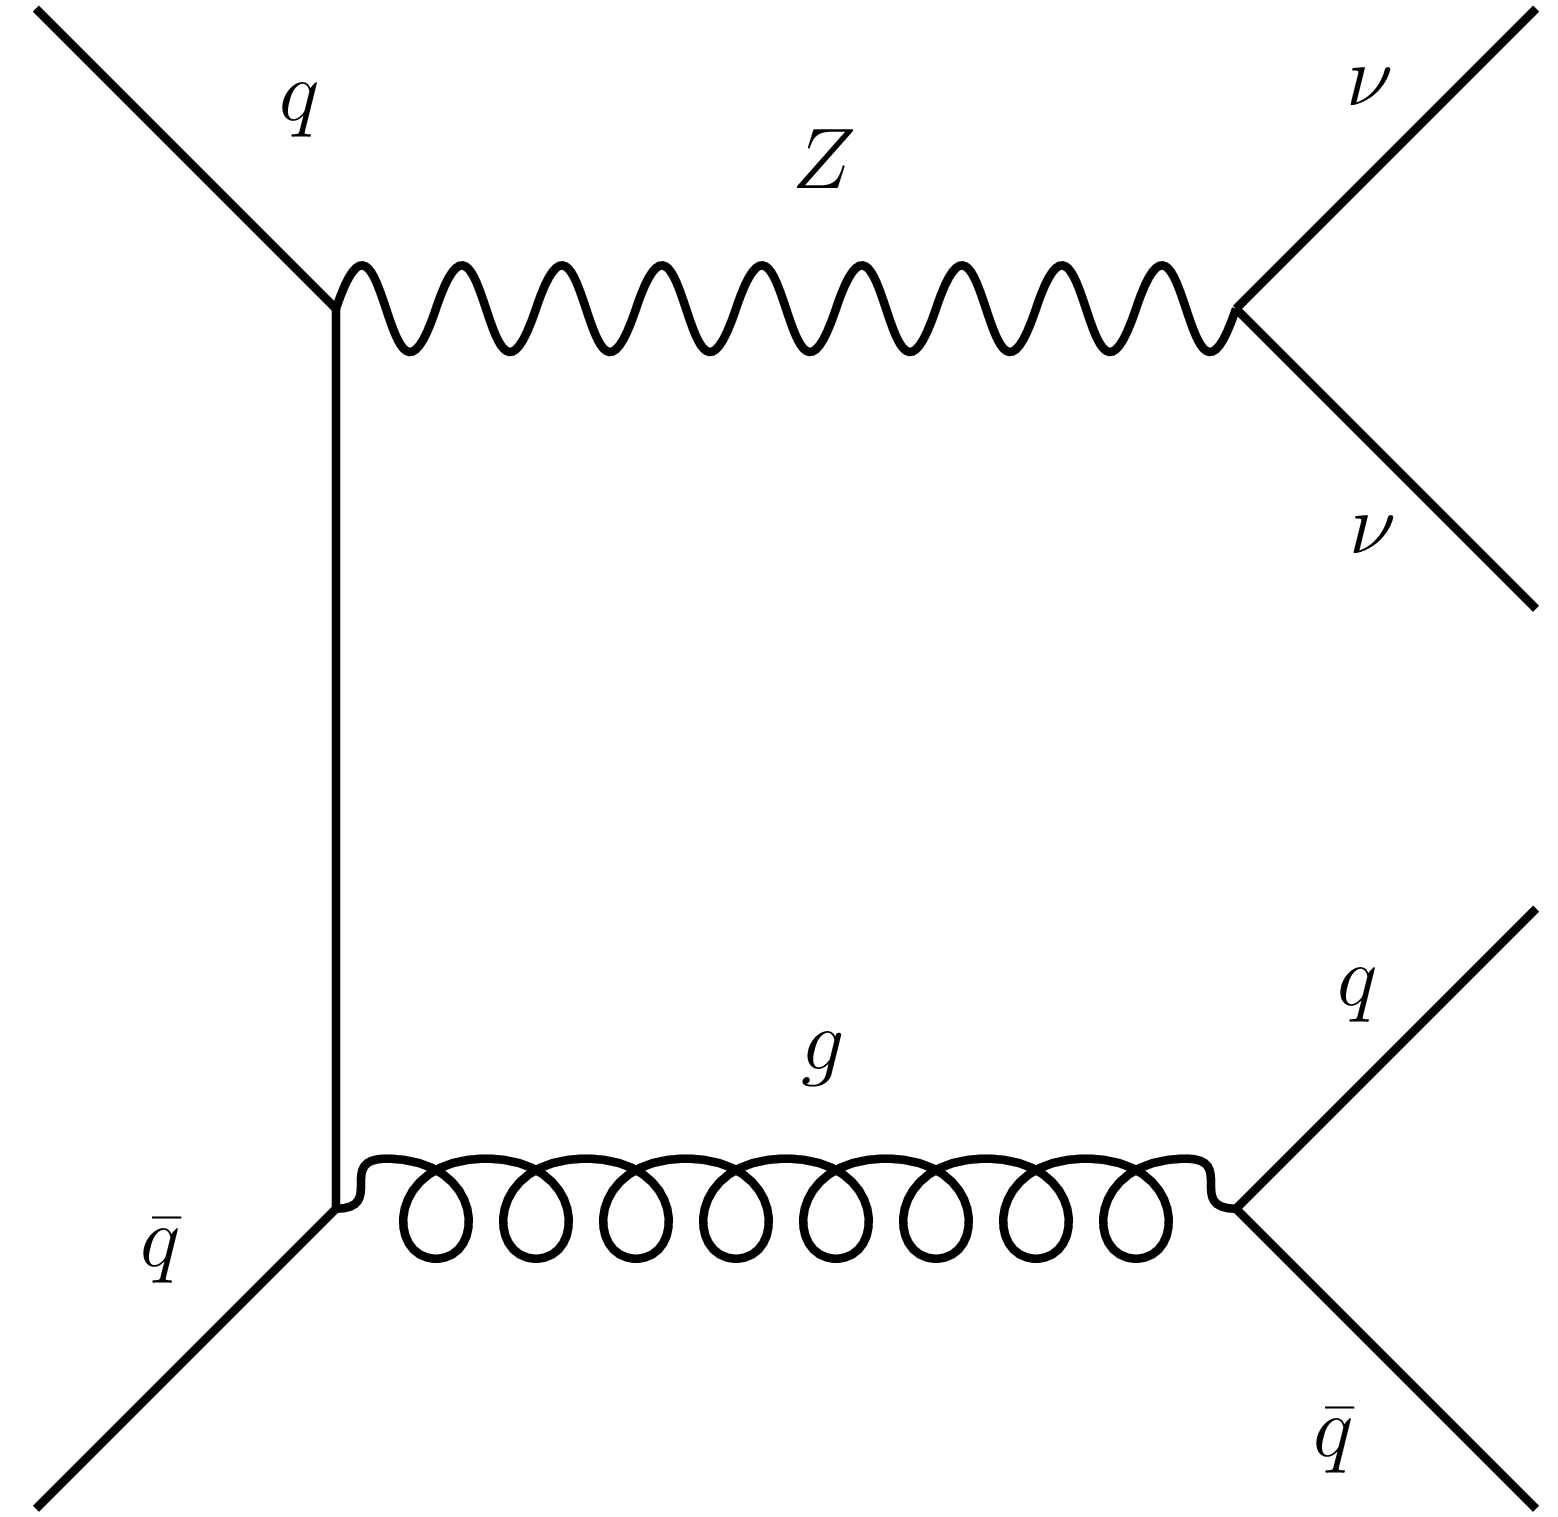
\includegraphics[width=0.3\linewidth]{Zvv.png}}
	~
	\subcaptionbox
	{$W$($l\nu$) + jets
		\label{fig:subfig_fig2}}
	{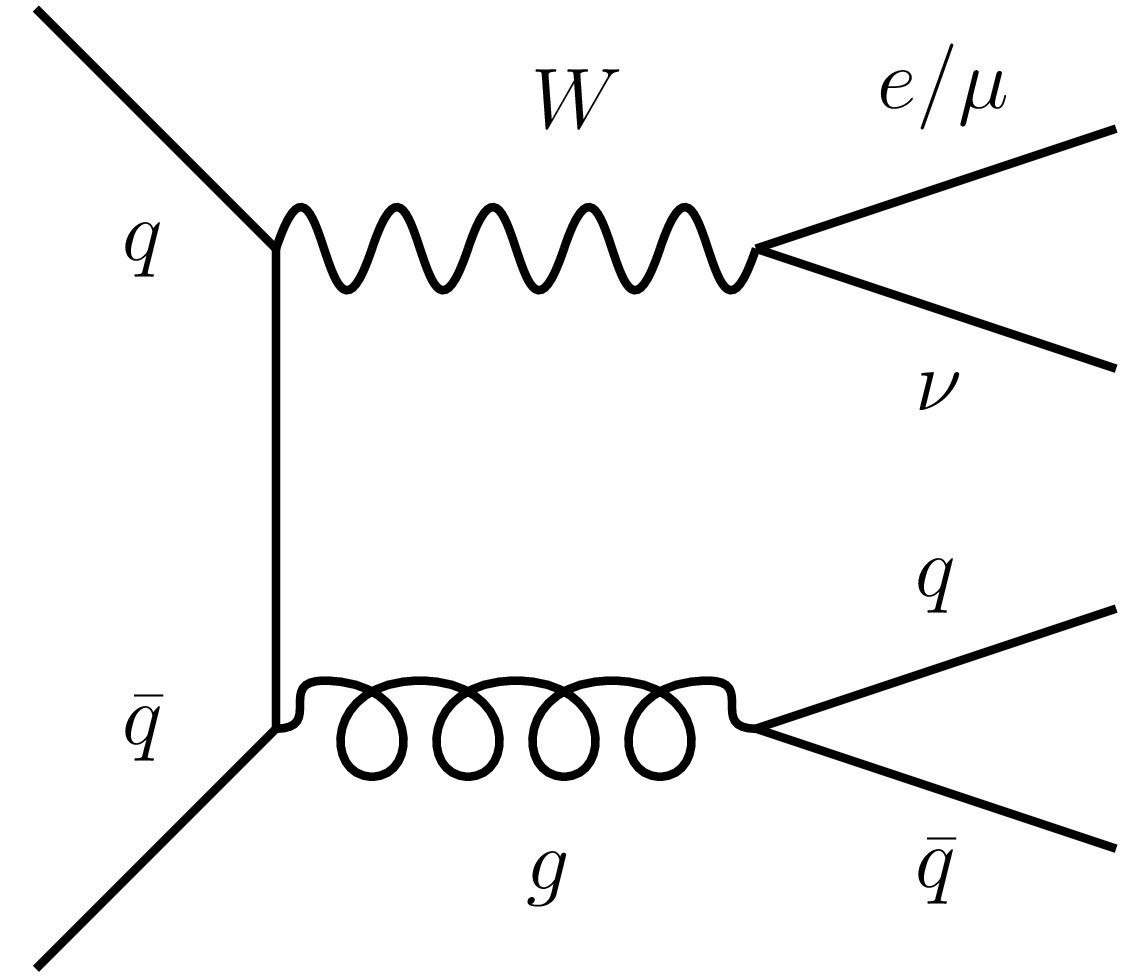
\includegraphics[width=0.3\linewidth]{Wlv.png}}
	~
	\subcaptionbox
	{$t\bar{t}$
		\label{fig:subfig_fig3}}
	{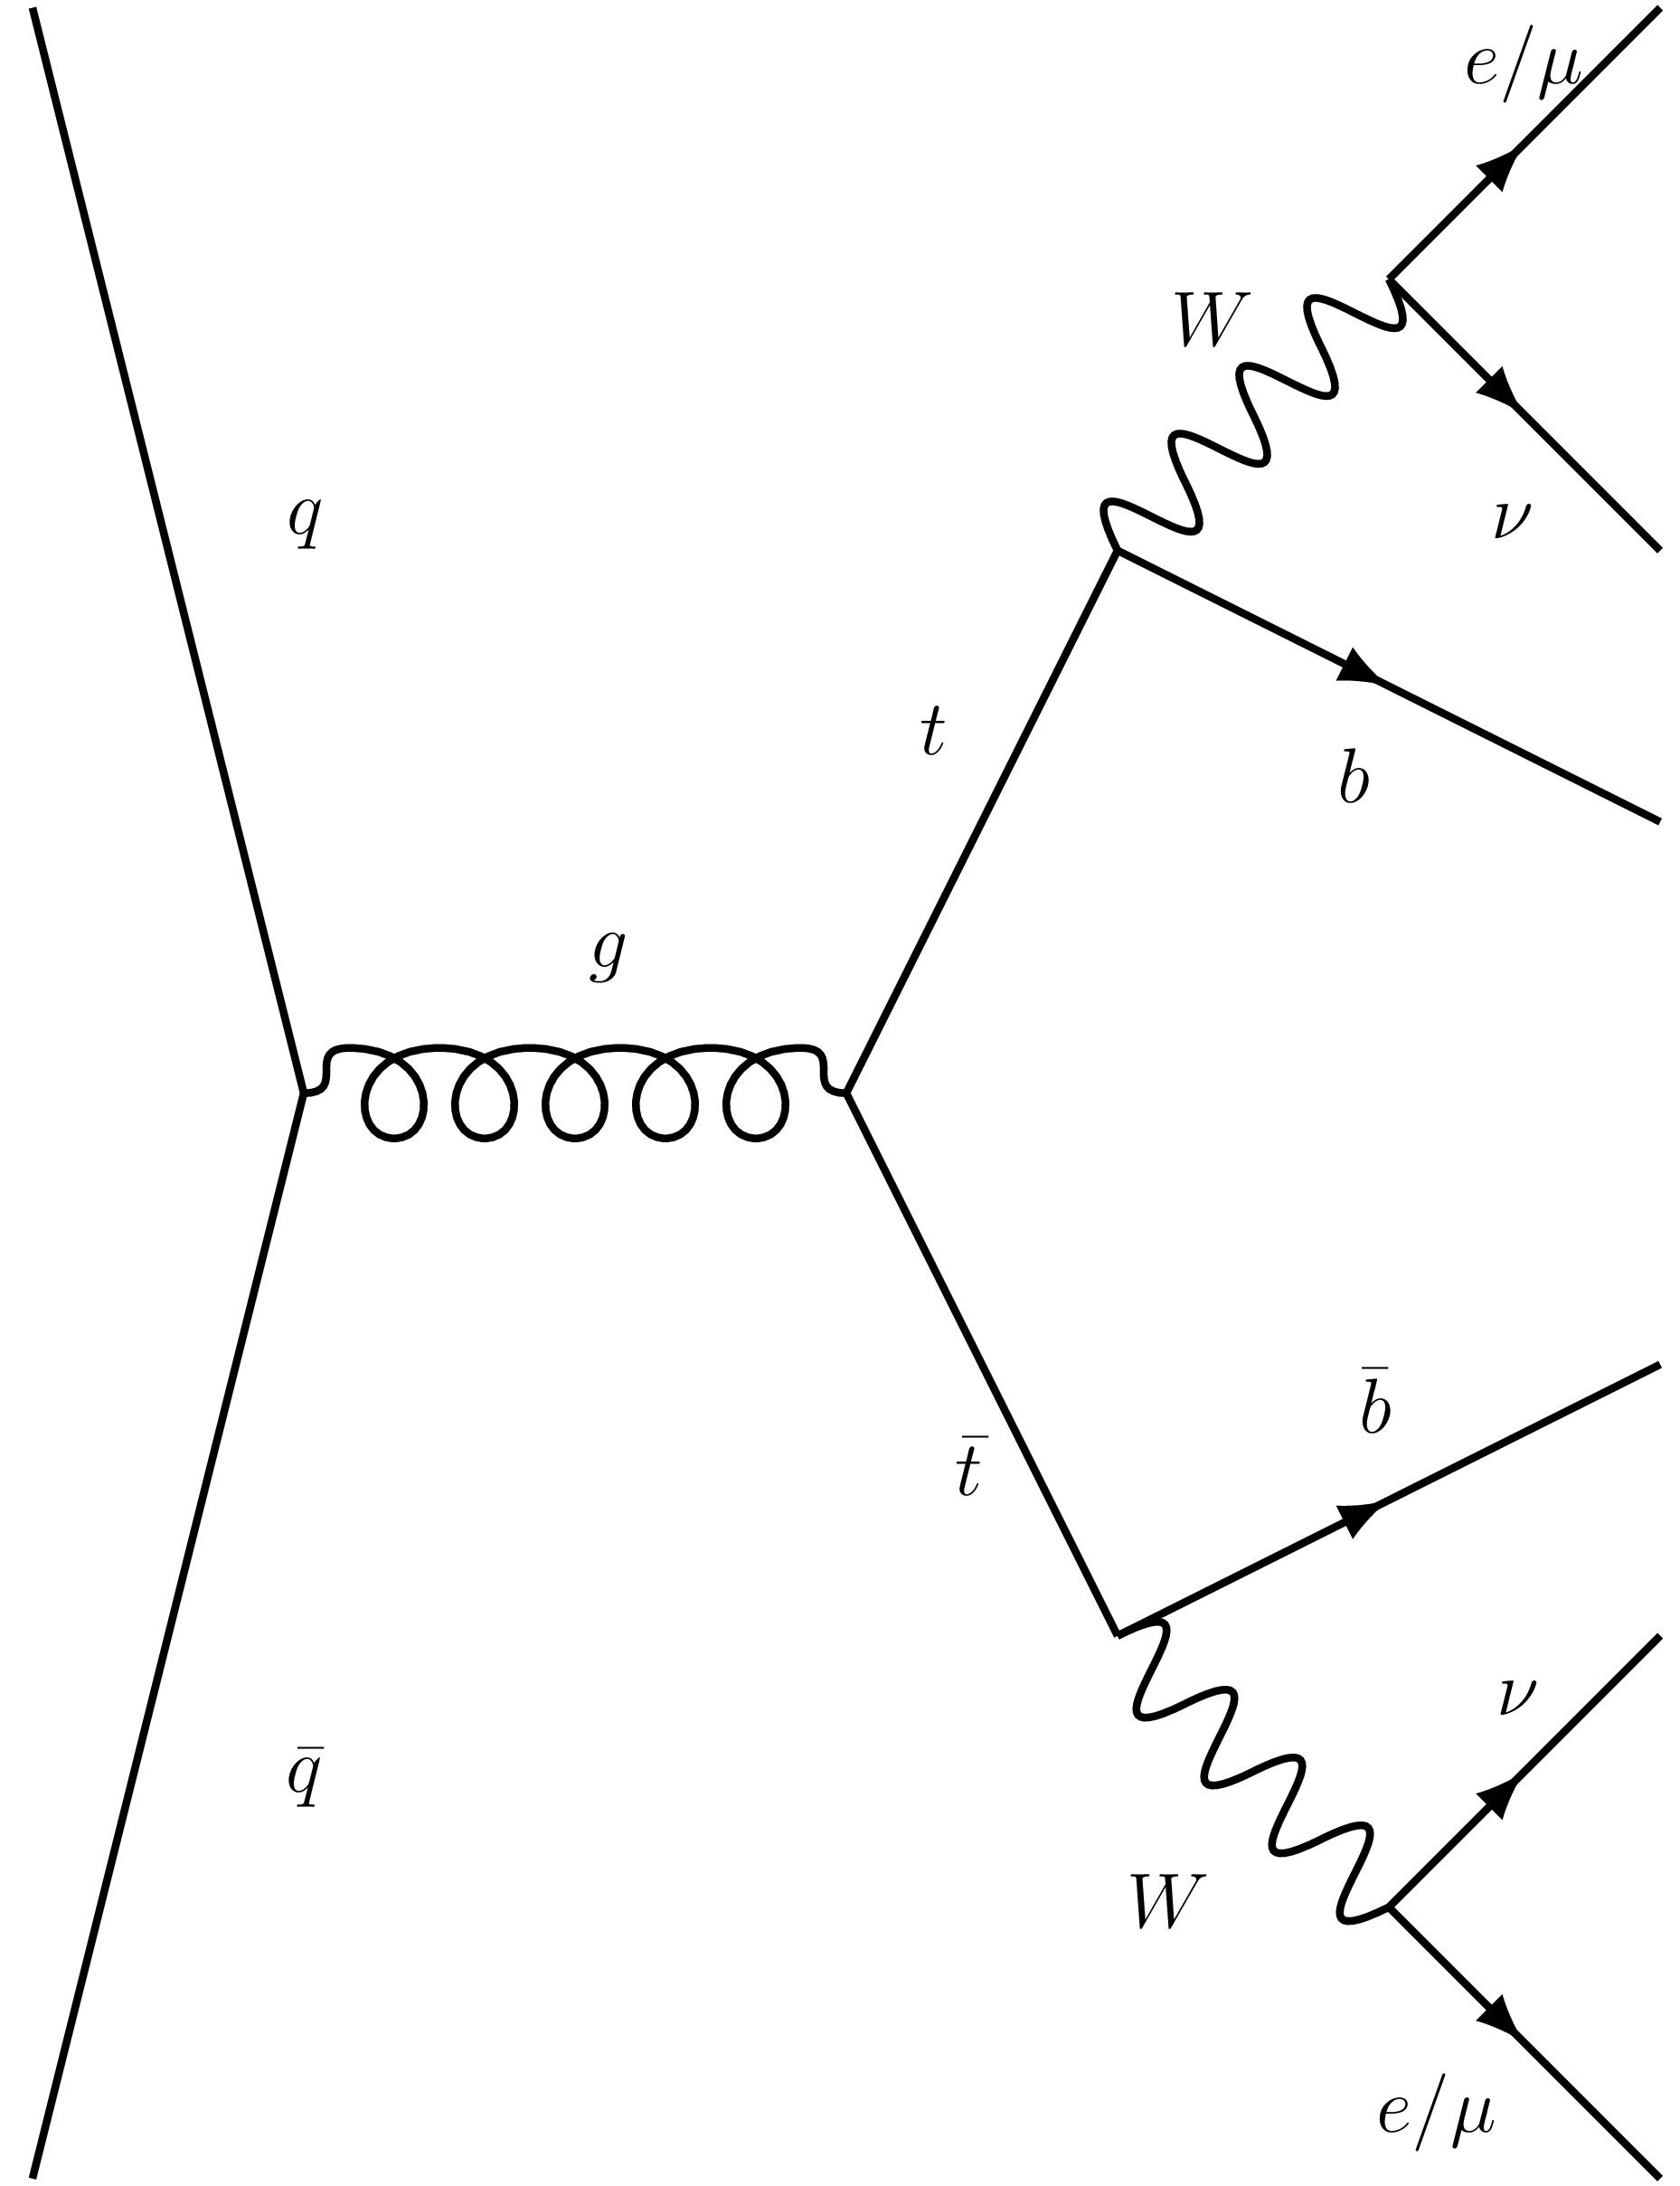
\includegraphics[width=0.3\linewidth]{ttbar.png}}
	\caption{The main background processes of the monoH analysis.}
	\label{fig:label}
\end{figure}

To constrain these background, the control region (CR) strategy is used. Before defining the CR, the signal region (SR) is defined as where the signals are expected to show. The SR is required to have no lepton based on the model. Then the CR is defined as the orthogonal region to the SR. Exploiting the similar kinematics, the CRs use some better-measured processes in order to constrain the background. There are two CRs in this analysis, the 1-lepton CR and the 2-lepton CR. The 1-lepton CR contains two processes, $W$($l\nu$) + jets and $t\bar{t}$, constraining the same processes in the SR. It requires different number of misidentified lepton, for $W$($l\nu$) + jets, one misidentified lepton in the SR but none in the 1-lepton CR, and for $t\bar{t}$, two misidentified leptons in the SR but one in the 1-lepton CR. The 2-lepton CR exploits the $Z$($ll$) + jets, constraining the $Z$($\nu\nu$) + jets process.

\section{Object Reconstruction and Selection}
\subsection{Jets}
Jets are a method to describe hadronic showers in detectors, consisting of multiple objects. Jets are reconstructed with the anti-$k_t$ algorithm. Depending on the toplogical clusters, the radius parameter of $R = 0.4$ is the small-radius (small-$R$) jets and of $R = 1.0$ is the large-radius (large-$R$) jets.

The small-$R$ jets with $p_T > 20 GeV$ for $\left|\eta\right| < 2.5$ are regarded to as the central jets. The MV2c10 discriminant is used for $b$-tagging the central jets to identify the $b$-hadrons, with the 77\% efficiency working point. In addition, the small-$R$ jets with $p_T > 30 GeV$ for $2.5 < \left|\eta\right| < 4.5$ are treated as the forward jets. The large-$R$ jets are required to have $p_T > 200 GeV$ and $\left|\eta\right| < 2.0$, containing multiple split jets called the track jets. The flavor identification for the large-$R$ jets depend on the ghost-associated track jets with the MV2c10 discriminant with the 77\% $b$-tagging efficiency working point. The track jets are depicted more in the following.

The fixed-radius (FR) track jets are applied for $b$-tagging in the previous analysis, using the anti-$k_t$ algorithm with fixed radius parameters. Instead of the FR track jets, the variable-radius (VR) track jets are implemented in the analysis for improving the $b$-tagging efficiency. The primary characteristic of the VR track jets is the relevance between the $p_T$ and the jet radius parameter: 
\begin{equation}
R \to R_{eff}(p_T) \approx \frac{\rho}{p_T}
\end{equation}
where $\rho$ is a constant factor. There are also two additional parameters, $R_{min}$ and $R_{max}$, as the radius boundary cut. The optimal values are respectively $\rho = 30 GeV$, $R_{min} = 0.02$ and $R_{max} = 0.4$.

\subsection{Leptons}
Electrons are reconstructed with energy deposits in the EM calorimeter which matches tracks in the ID. Besides the basic reconstruction, there are two types of electrons for the further selection in the analysis, the baseline electrons and the signal electrons. The baseline electrons have a loose criterion with $\left|\eta\right| < 2.47$ and $p_T < 7 GeV$, used for electron vetoes. For the events containing electrons, the signal electrons require $\left|\eta\right| < 2.47$ and $p_T < 27 GeV$.

The muon reconstruction relies on the muon spectrometer in the range of $\left|\eta\right| < 2.7$. It's also claimed to match the tracks in the ID for $\left|\eta\right| < 2.5$. Like electrons, there are two categories of muons, the baseline muons and the signal muons. The baseline muons are used for vetoing events in certain regions, requiring $\left|\eta\right| < 2.7$ and $p_T < 7 GeV$. The signal muons are defined with the criterion of $\left|\eta\right| < 2.5$ and $p_T < 25 GeV$ for the events which contain muons.

Because of the hadronic-like nature of taus, the reconstruction is complicated and described in Reference[]. For the tau vetoes in the analysis, the taus are required to have one or three tracks and have $\left|\eta\right| < 2.5$ and $p_T < 20 GeV$, excluding the crack region $1.37 < \left|\eta\right| < 1.52$.

\subsection{Missing Transverse Momentum}
The missing transverse momentum is determined as the negative vector sum of the transverse momentum of all the reconstructed and calibrated objects in an event. Additionally, the track-based soft term is added into the missing transverse momentum in the analysis, which is from the tracks that not associated with any reconstructed object but still linked to the primary vertex. The absolute value of the missing transverse momentum is expressed as $E^{miss}_T$, or MET. Also, there is a purely track-based missing transverse momentum calculated as the negative vector sum of the transverse momentum of all the reconstructed tracks associated with the primary vertex. The absolute value of the track-based missing transverse momentum is denoted as $p^{miss}_T$.

Furthermore, to recognize whether the MET is from weakly interacting particles or from the mismeasurement of multijet processes, two kinds of the MET significance are applied. One is the event-based MET significance which is performed in previous monoHbb analysis, and the other is the object-based MET significance which is newly introduced in the analysis. They will be depicted more detailed in the following section.

\section{Event Selection}
The SR is divided into two parts, the resolved region ($150 < E^{miss}_T < 500 GeV$) and the merged region ($E^{miss}_T > 500 GeV$), for different event selection requirements. As previously mentioned in 3.2, to be the comparison of the SR, the CRs are also divided into two divisions with the $p_T$ of the vector boson ($W$ or $Z$) as the separation boundary ($150 < p^V_T < 500 GeV$ for the resolved region and $p^V_T > 500 GeV$ for the merged region). The common selection among the SR and the CRs is introduced before the respective selection. The total event selection will be summarized in Table 1.

\subsection{Common Selection}


\subsection{Respective Selection}

MET sig

\section{Systematic Uncertainty}

\section{Results}
the improvement of this analysis
VR
object-based MET sig

\end{document}          % 實驗結果
        \documentclass[class=NTHU_thesis, crop=false]{standalone}
\begin{document}

\chapter{Conclusion}
\label{chap:Conclusion}
I am free, I am not own by M\${}.

\end{document}      % 結論
        \documentclass[class=NTHU_thesis, crop=false]{standalone}
\begin{document}

\chapter{Chapter name(demo)}
Content of chapter \\
Content Content Content.

\section{Section name}
Content of section \\
Content Content Content
\subsection{Subsection name}
Content of subsection \\
Content Content Content

\subsubsection{Subsubsection name}
Content of subsubsection \\
Content Content Content

\paragraph{Paragraph name}
Content of paragraph \\
Content Content Content

\subparagraph{Subparagraph name}
Content of subparagraph \\
Content Content Content


\chapter{Test demo}
First line.
(next line in \LaTeX\ )still first line. \\
Second line.


\chapter{figure}
\section{Insert single figure(by sppmg's tool)}
\fig[0.15][fig:label_test][!hbt]{logo-Linux.png}[caption][short caption]

\section{Insert figures}
\begin{figure}[!hbt]
    %\captionsetup[subfigure]{labelformat=empty} % hide figure's number.
    \centering
    \subcaptionbox
        {caption\_1
        \label{fig:subfig_fig1}}
        {
\includegraphics[width=0.3\linewidth]{fig1.png}}
    ~
    \subcaptionbox
        {caption\_2
        \label{fig:subfig_fig2}}
        {
\includegraphics[width=0.3\linewidth]{fig2.eps}}
    \vspace{\baselineskip} % 分隔上下列
    \subcaptionbox
        {caption\_3
        \label{fig:subfig_fig3}}
        {
\includegraphics[width=0.6\linewidth]{fig3.png}}
    \caption{caption, use ``\subref{fig:subfig_fig2}'' get ID of subfigure(this ID is Debian) in caption}
    \label{fig:label}
\end{figure}


\chapter{Table}
\section{Simple table}
\begin{table}[h]
    \centering
    \caption{Solution}
    \begin{tabular}{| l | l |}
        \hline
        Component  & Concentration(mM) \\ \hline
        \ce{CaCl2} & 118.0 \\ \hline
    \end{tabular}
\end{table}

\section{Auto break line table}
\begin{table}[h]
    \centering
    \begin{tabularx}{\textwidth}{| l | X |}
        \hline
        short & short short \\ \hline
        long  & long long long long long long long long long long \\ \hline
    \end{tabularx}
\end{table}

\end{document}
    \backmatter          % book class 預設\backmatter 在\appendix 後面。因此.cls修改過\appendix 定義
        % This file has 3 types bibliography management, 
% \bibManType in config.tex choose it.
% 0. Embedded: write \bibitem in {thebibliography} environment.
% 1. BibTeX: Change bib files in \bibliography{}
% 2. biber / BibLaTeX: Add bibliography by \addbibresource{bibfile.bib} in macros_preamble.tex

\documentclass[class=NTHU_thesis, crop=false]{standalone}

\begin{document}

\ifcase \bibManType 
    % 0 == Embedded %%%%%%%%%%%%%%%%%%%%%%%%%%%%%%%%%%%%%%%
    {\bibFontStyle\setstretch{\bibLineStretch}
    \begin{thebibliography}{99}

    \bibitem{cite_key_1}
        bibliography item detail.

    \bibitem{_sppmg/tw_thesis_template_????}
        TW\_Thesis\_Template,
        sppmg,
        \url{https://github.com/sppmg/TW_Thesis_Template},
        Embedded bibliography demo.

    \end{thebibliography}
    }
    
\or
    % 1 == BibTeX %%%%%%%%%%%%%%%%%%%%%%%%%%%%%%%%%%%%%%%%%
    \bibliographystyle{\bibStyle}
    {\bibFontStyle\setstretch{\bibLineStretch}
        \bibliography{demo} % {sample_1,sample_2,...,sample_n}
        % Note the lack of whitespace between the commas and the next bib file.
    }
\or

    % 2 == biber / BibLaTeX %%%%%%%%%%%%%%%%%%%%%%%%%%%%%%%
    \printbibliography[heading = bibnumbered, title = {Reference}]
\fi



\end{document}
    \appendix
        \documentclass[class=NTHU_thesis, crop=false]{standalone}
\begin{document}

\chapter{List of device}

\begin{table}[!h]
    \centering
    \begin{tabularx}{\textwidth}{|l|l|X|}
        \hline
        device  & Model    & Description \\ \hline
        Linux   & Debian 9 & Best of best of best OS \\ \hline
        Windows & 10       & Best of Best tool to prevent the aging of brain. \\ \hline
    \end{tabularx}
    \caption{List of device}
    \label{table:list_device}
\end{table}

\end{document}
        \documentclass[class=NTHU_thesis, crop=false]{standalone}
\begin{document}

\definecolor{Gray3}{gray}{0.8}

\chapter{Solutions}

\section{The solution}
\begin{table}[!h]
    \centering
    \begin{tabular}{| l | l |}
        \hline
        Component & Concentration(mM) \\ \hline
        \rowcolor{Gray3}
        \ce{NaCl} & 1.0 \\ \hline
        \ce{CaCl_2} & 2.0 \\ \hline
        \rowcolor{Gray3}
        \ce{NaCl} & 1.0 \\ \hline
        \ce{CaCl_2} & 2.0 \\ \hline
    \end{tabular}
    \caption{The solution}
\end{table}
\end{document}
        \documentclass[class=NTHU_thesis, crop=false]{standalone}
\begin{document}
% Here demo instert whole code file. You can only insert code directly, 
% please read my tutorial or document of listings package.
% code style set in macros_preamble already.
% Supported language please read document of listings package.


\chapter{Code}
\section{C}
\lstinputlisting[language=C]{hello_world_c.c}

\section{Matlab}
\lstinputlisting[language=matlab]{hello_world_matlab.m}

\section{IDL}
\lstinputlisting[language=IDL]{hello_world_idl.pro}
\end{document}

%         \documentclass[class=NTHU_thesis, crop=false]{standalone}

\begin{document}
\chapter{Letters bot}

Here try to insert some information automatically.
If you need change font size or position, modify appendix\_letter\_NCU.tex and compile this single tex file.

In appendix\_letter\_NCU.tex, you will see \textbackslash{}placetextbox for every string.
\begin{lstlisting}[style=LatexStyle,caption={}]
\placetextbox{x(mm)}{y(mm)}
\end{lstlisting}

The unit is mm , origin at bottom left. I recommend add ``colorgrid'' option to ``\textbackslash{}documentclass'' for positioning. e.g. In this tex file (appendix\_letter\_NCU.tex):

\begin{lstlisting}[style=LatexStyle,caption={}]
\documentclass[class=NTHU_thesis, crop=false, colorgrid]{standalone}
\end{lstlisting}

``colorgrid'' will display a grid with mm unit. 

\begin{center}
{ \noindent\color{red}\bfseries\Large NCU 中文文件位於 NCU\_zh}
\end{center}

%%%%%%%%%%%%%%%%%%%%%%%%%%%%%%%%
% define \mprof 
\ExplSyntaxOn
    % Copy prof. list from config.tex
    \clist_gclear_new:N \g_sppmg_profs_cl
    \clist_gset:NV \g_sppmg_profs_cl \profs
    \clist_gpop:NNTF \g_sppmg_profs_cl \l_tmpa_tl {}{ \tl_clear:N \l_tmpa_tl}
    \cs_gset_eq:NN \mprof \l_tmpa_tl
\ExplSyntaxOff

% Define local variable (e.g. cover use \titleZh for \title but letters use \titleEn )
\def\title{\titleEn}

%%%%%%%%%%%%%%%%%%%%%%%%%%%%%%%%
\cleardoublepage
\pagestyle{empty}
\sffamily
% ------------------------------

% 碩博士論文電子檔授權書
\IfFileExists{\letterAuthEl}{
\cleardoublepage\thispagestyle{empty}
\includepdf[pagecommand={   \placetextbox{115}{87}{\fs{14}\title}%
                            \placetextbox{100}{81}{\fs{14}\mprof}%
                            \placetextbox{85}{70}{\fs{14}\deptshort} }]%
{\letterAuthEl}}{}

% 碩博士紙本論文延後公開/下架申請書。(如需延後公開者,才需要裝訂於論文內頁)
\IfFileExists{\letterPubReq}{
\cleardoublepage\thispagestyle{empty}
\includepdf[pagecommand={   \placetextbox{128}{269}{\fs{14}\author}%
                            \placetextbox{70}{255}{\fs{14}\deptshort}%
                            \placetextbox{100}{231}{\fs{14}\title}%
                            \placetextbox{90}{218.3}{\fs{14}\mprof} }]%
{\letterPubReq}}{}

% 指導教授推薦書
\IfFileExists{\letterRecom}{
\cleardoublepage\thispagestyle{empty}
\includepdf[pagecommand={   \placetextbox{75}{204}{\fs{16}\deptshort}%
                            \placetextbox{90}{218}{\fs{16}\author}%
                            \placetextbox{105}{192}{\fs{16}\title}}%
]{\letterRecom}}{}

% 口試委員審定書
\IfFileExists{\letterVerif}{
\cleardoublepage\thispagestyle{empty}
\includepdf[pagecommand={   \placetextbox{75}{184}{\fs{16}\deptshort}%
                            \placetextbox{91}{200}{\fs{16}\author}%
                            \placetextbox{100}{170}{\fs{16}\title}}%
]{\letterVerif}}{}

% ------------------------------
\pagestyle{fancy}
\end{document}
\end{document}